\documentclass[a4paper, 12pt]{article}
\usepackage{temp}
\usepackage{epsfig,graphicx,subfigure,amsthm,amsmath, float, xcolor, changepage, mathtools, textcomp, hyperref, bm, amssymb, tcolorbox, tikz, setspace}
\usepackage{array}
\usepackage[shortlabels]{enumitem}
\usepackage[stable]{footmisc}
\usepackage{xepersian}
\settextfont[Scale=1]{XBZar}
%\setdigitfont{XBZar}
\setlatintextfont[Scale=0.9]{Times New Roman}
\hypersetup{
	colorlinks=true,
	urlcolor=blue!70!black
}
\definecolor{darkpastelgreen}{rgb}{0.01, 0.75, 0.24}


\doublespacing
\begin{document}
\handout
{هوش مصنوعی}
{نیم‌سال اول ۰۱\lr{-}۰۰}
{دکتر محمدحسین رهبان}
{دانشکده مهندسی کامپیوتر}
{تمرین هفتم - بخش اول}
{محمدجواد هزاره}
{98101074}
\noindent
\\[-6.5em]
\section*{سوال ۱}
برای مدل‌سازی سه حالت زیر را در نظر می‌گیریم. با توجه به تقارن، هر حالت دیگری را می‌توان به شکل یکی از این سه حالت در نظر گرفت. \lr{G} نشان دهنده‌ی مکان روح و \lr{P} مکان پک‌من را نشان می‌دهد.
\begin{center}
	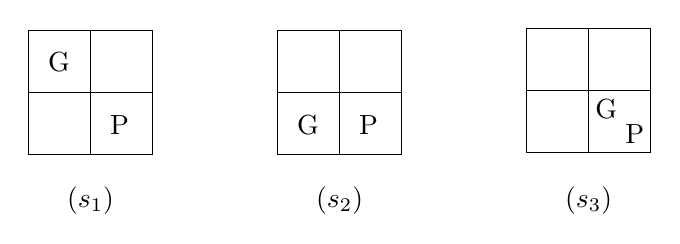
\begin{tikzpicture}[x=0.75pt,y=0.75pt,yscale=-1,xscale=1]
		%uncomment if require: \path (0,300); %set diagram left start at 0, and has height of 300
		
		%Shape: Grid [id:dp6197727097433838] 
		\draw  [draw opacity=0] (179,121) -- (239,121) -- (239,181) -- (179,181) -- cycle ; \draw   (209,121) -- (209,181) ; \draw   (179,151) -- (239,151) ; \draw   (179,121) -- (239,121) -- (239,181) -- (179,181) -- cycle ;
		%Shape: Grid [id:dp18663832830724947] 
		\draw  [draw opacity=0] (299,121) -- (359,121) -- (359,181) -- (299,181) -- cycle ; \draw   (329,121) -- (329,181) ; \draw   (299,151) -- (359,151) ; \draw   (299,121) -- (359,121) -- (359,181) -- (299,181) -- cycle ;
		%Shape: Grid [id:dp40469079628764937] 
		\draw  [draw opacity=0] (419,120) -- (479,120) -- (479,180) -- (419,180) -- cycle ; \draw   (449,120) -- (449,180) ; \draw   (419,150) -- (479,150) ; \draw   (419,120) -- (479,120) -- (479,180) -- (419,180) -- cycle ;
		
		% Text Node
		\draw (193.84,136.5) node [align=left] {\lr{G}};
		% Text Node
		\draw (223.01,166.5) node [align=left] {\lr{P}};
		% Text Node
		\draw (209,195) node [anchor=north] [inner sep=0.75pt] {$(s_{1})$};
		% Text Node
		\draw (313.84,166.5) node [align=left] {\lr{G}};
		% Text Node
		\draw (343.01,166.5) node [align=left] {\lr{P}};
		% Text Node
		\draw (329,195) node [anchor=north] [inner sep=0.75pt] {$(s_{2})$};
		% Text Node
		\draw (451,153) node [anchor=north west][inner sep=0.75pt] [align=left] {\lr{G}};
		% Text Node
		\draw (477,177) node [anchor=south east] [inner sep=0.75pt] [align=left] {\lr{P}};
		% Text Node
		\draw (449,195) node [anchor=north] [inner sep=0.75pt] {$(s_{3})$};
	\end{tikzpicture}
\end{center}
اگر فرض کنیم روح همواره به نحوی حرکت خواهد کرد که فاصله‌اش را با پک‌من کم کند، آن‌گاه برای مدل‌سازی مسئله خواهیم داشت: (برای هر یال، حرکت پک‌من و بلافاصله بهترین حرکت روح در نظر گرفته شده است.) \lr{reward} مربوط به یال‌های منتهی به $s_1$ و $s_2$ برابر با $1$ و سایر یال‌ها $0$ خواهد بود.
\begin{center}
	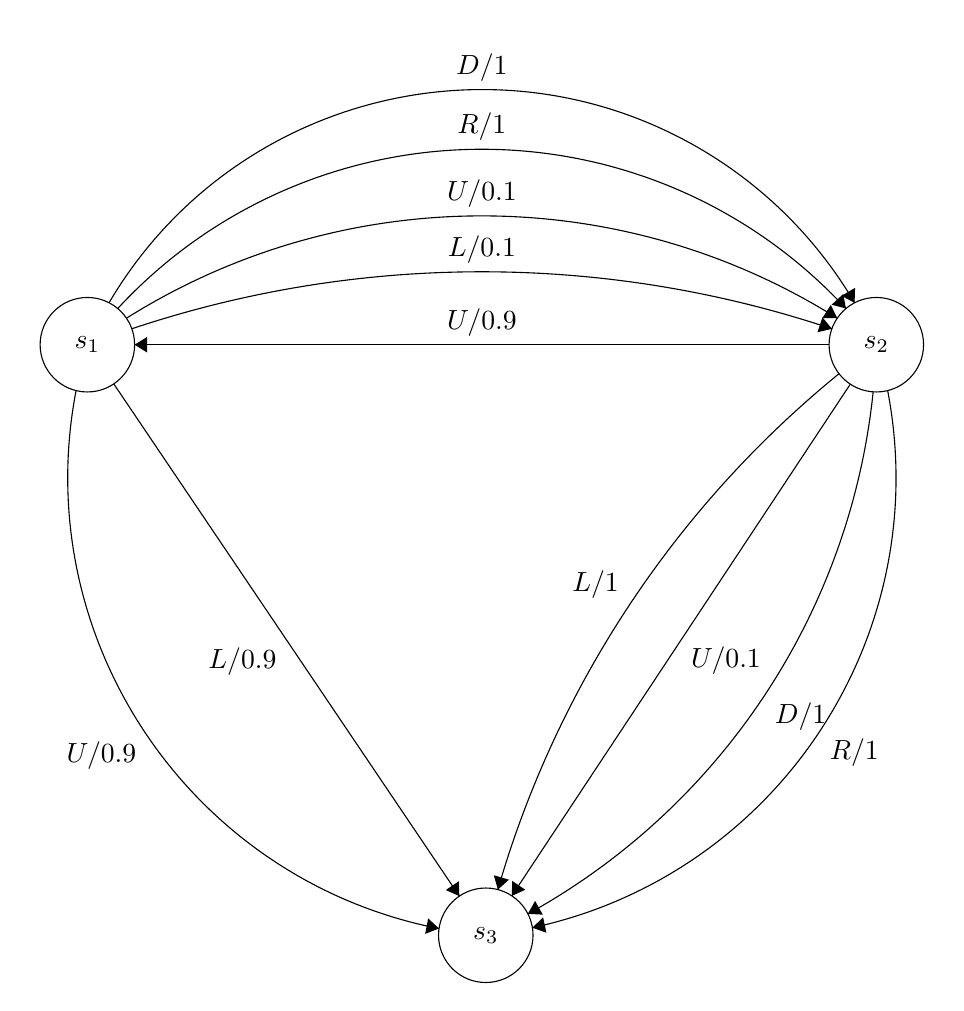
\begin{tikzpicture}[scale=0.2]
		\tikzstyle{every node}+=[inner sep=0pt]
		\draw [black] (14.8,-18.4) circle (3);
		\draw (14.8,-18.4) node {$s_1$};
		\draw [black] (64.9,-18.4) circle (3);
		\draw (64.9,-18.4) node {$s_2$};
		\draw [black] (40.1,-55.9) circle (3);
		\draw (40.1,-55.9) node {$s_3$};
		\draw [black] (17.624,-17.387) arc (108.50272:71.49728:70.037);
		\fill [black] (62.08,-17.39) -- (61.48,-16.66) -- (61.16,-17.61);
		\draw (39.85,-13.27) node [above] {$L/0.1$};
		\draw [black] (17.282,-16.716) arc (122.12957:57.87043:42.434);
		\fill [black] (62.42,-16.72) -- (62.01,-15.87) -- (61.47,-16.71);
		\draw (39.85,-9.72) node [above] {$U/0.1$};
		\draw [black] (37.132,-55.475) arc (-101.09554:-190.89201:29.193);
		\fill [black] (37.13,-55.47) -- (36.44,-54.83) -- (36.25,-55.81);
		\draw (17.94,-44.5) node [left] {$U/0.9$};
		\draw [black] (16.48,-20.89) -- (38.42,-53.41);
		\fill [black] (38.42,-53.41) -- (38.39,-52.47) -- (37.56,-53.03);
		\draw (26.84,-38.49) node [left] {$L/0.9$};
		\draw [black] (16.728,-16.103) arc (137.25537:42.74463:31.484);
		\fill [black] (62.97,-16.1) -- (62.8,-15.18) -- (62.06,-15.86);
		\draw (39.85,-5.49) node [above] {$R/1$};
		\draw [black] (16.177,-15.737) arc (149.52484:30.47516:27.467);
		\fill [black] (63.52,-15.74) -- (63.55,-14.79) -- (62.69,-15.3);
		\draw (39.85,-1.7) node [above] {$D/1$};
		\draw [black] (40.866,-53) arc (163.90169:129.14232:65.744);
		\fill [black] (40.87,-53) -- (41.57,-52.37) -- (40.61,-52.09);
		\draw (48.58,-33.63) node [left] {$L/1$};
		\draw [black] (65.618,-21.311) arc (10.91098:-77.86696:29.23);
		\fill [black] (43.06,-55.42) -- (43.95,-55.74) -- (43.74,-54.76);
		\draw (61.91,-44.3) node [right] {$R/1$};
		\draw [black] (64.698,-21.393) arc (-5.87101:-61.08497:42.882);
		\fill [black] (42.77,-54.54) -- (43.72,-54.59) -- (43.23,-53.72);
		\draw (58.42,-41.99) node [right] {$D/1$};
		\draw [black] (61.9,-18.4) -- (17.8,-18.4);
		\fill [black] (17.8,-18.4) -- (18.6,-18.9) -- (18.6,-17.9);
		\draw (39.85,-17.9) node [above] {$U/0.9$};
		\draw [black] (63.25,-20.9) -- (41.75,-53.4);
		\fill [black] (41.75,-53.4) -- (42.61,-53.01) -- (41.78,-52.45);
		\draw (53.11,-38.48) node [right] {$U/0.1$};
	\end{tikzpicture}
\end{center}
\begin{enumerate}[A)]
	\item
	اگر داشته باشیم
	$x \in \{D, R\}$
	،
	$y \in \{U, L\}$
	،
	$z \in \{U\}$
	و
	$w \in \{D, L, R\}$
	،
	با توجه به گراف مسئله، ارزش سیاست ما نه به خود اکشن‌ها بلکه به دسته‌ای که اکشن را از آن انتخاب می‌کنیم بستگی خواهد داشت. حال سیاست زیر را در نظر می‌گیریم:
	\[
	\pi^{\ast} = \begin{dcases}
		s_1 \to x \\
		s_2 \to z
	\end{dcases}
	\]
	حالت $s_3$ نیز کنشی نخواهد داشت. ادعا می‌کنیم این سیاست خواسته‌ی مسئله را برآورده می‌کند. به عبارتی به ازای هر سیاست $\pi$، خواهیم داشت
	$\pi^\ast \ge \pi$.
	با توجه به تعریفی که برای
	$x$، $y$، $w$ و $z$
	داشتیم، سه حالت دیگر برای $\pi$ باقی می‌ماند که به صورت زیر هستند:
	\[
	\pi_1 = \begin{dcases}
		s_1 \to x \\
		s_2 \to w
	\end{dcases} \qquad \quad
	\pi_2 = \begin{dcases}
		s_1 \to y \\
		s_2 \to z
	\end{dcases} \qquad \quad
	\pi_3 = \begin{dcases}
		s_1 \to y \\
		s_2 \to w
	\end{dcases}
	\]
	با حل معادلات تابع ارزش برای هر یک از این سیاست‌ها خواهیم داشت:
	\[
	V^{\pi^\ast} = \left[\begin{array}{c}
		\frac{1+0.9\gamma}{1-0.9\gamma^2} \\
		0.9\frac{1+\gamma}{1-0.9\gamma^2}
	\end{array}\right]
	\qquad V^{\pi_1} = \left[\begin{array}{c}
		1 \\
		0
	\end{array}\right]
	\qquad V^{\pi_2} = \left[\begin{array}{c}
		0.1\frac{1+0.9\gamma}{1-0.09\gamma^2} \\
		0.9\frac{1+0.1\gamma}{1-0.09\gamma^2}
	\end{array}\right]
	\qquad V^{\pi_3} = \left[\begin{array}{c}
		0.1 \\
		0
	\end{array}\right]
	\]
	که اگر $\gamma$ عددی مثبت و کوچک‌تر از $1$ باشد، مشخص است که $\pi^\ast$ از
	$\pi_1$
	و
	$\pi_3$
	بهتر است. هم‌چنین از $\pi_2$ بهتر خواهد بود که برای اثبات آن می‌توان به نمودار‌های زیر دقت کرد:
	{\scriptsize (\textcolor{red}{$0.9\frac{1+\gamma}{1-0.9\gamma^2}$}
	\textcolor{orange}{$0.9\frac{1+0.1\gamma}{1-0.09\gamma^2}$},
	\textcolor{blue}{$\frac{1+0.9\gamma}{1-0.9\gamma^2}$},
	\textcolor{darkpastelgreen}{$0.1\frac{1+0.9\gamma}{1-0.09\gamma^2}$}) }
	\begin{figure}[H]
		\centering
		\includegraphics[width=0.3\textwidth]{7-1-1.png}
		\hspace*{2cm}
		\includegraphics[width=0.3\textwidth]{7-1-2.png}
	\end{figure}
	\item
	با توجه به قسمت قبل، سیاست زیر خواسته‌ی مسئله را برآورده می‌کند:
	\[
	\pi^{\ast}_{\text{det}} = \begin{dcases}
		s_1 \to D \\
		s_2 \to U
	\end{dcases}
	\]
\end{enumerate}
\end{document}



